\documentclass[8pt, letterpaper, titlepage]{article}
\usepackage[utf8]{inputenc}
\usepackage{geometry}
\usepackage{color,graphicx,overpic} 
\usepackage{fancyhdr}
\usepackage{amsmath,amsthm,amsfonts,amssymb}
\usepackage{mathtools}
\usepackage{hyperref}
\usepackage{multicol}
\usepackage{array}
\usepackage{float}
\usepackage{blindtext}
\usepackage{longtable}
\usepackage{scrextend}
\usepackage[font=small,labelfont=bf]{caption}
\usepackage[framemethod=tikz]{mdframed}
\usepackage{calc}
\usepackage{titlesec}
\usepackage{listings}
\usepackage[normalem]{ulem}
\usepackage{tabularx}
\usepackage{mathrsfs}
\usepackage{bookmark}
\usepackage{setspace}
\usepackage{tabularx}
\usepackage{ltablex}
\usepackage{enumitem}
\usepackage[simplified]{pgf
-umlcd}
\definecolor{dkgreen}{rgb}{0,0.6,0}
\definecolor{gray}{rgb}{0.5,0.5,0.5}
\definecolor{mauve}{rgb}{0.58,0,0.82}
\usepackage{listings}

\lstset{frame=tb,
  language=Java,
  aboveskip=3mm,
  belowskip=3mm,
  showstringspaces=false,
  columns=flexible,
  basicstyle={\small\ttfamily},
  numbers=none,
  numberstyle=\tiny\color{gray},
  keywordstyle=\color{blue},
  commentstyle=\color{dkgreen},
  stringstyle=\color{mauve},
  breaklines=false,
  breakatwhitespace=true,
  tabsize=3
}

\mathtoolsset{showonlyrefs}  
\allowdisplaybreaks

\definecolor{mycolor}{rgb}{0, 0, 0}

\geometry{top=2.54cm, left=2.54cm, right=2.54cm, bottom=2.54cm}

% Indentation/space between paragraphs
\setlength{\headheight}{15pt}
\setlength{\parindent}{0pt}
\setlength{\parskip}{0pt}

% Line spacing
\renewcommand{\baselinestretch}{1.5} 

% Line spacing
\renewcommand{\baselinestretch}{1.3} 

% Title page
\title{\textbf{\Huge{ 
\begin{center}
MATE 201\\ \large{Class notes} % Document name
\end{center} 
}}}

\author{Lora Ma}

% Header/Footer
\pagestyle{fancy}
\fancyhf{}
\rhead{\thepage}
\lhead{\textit{CMPUT 366 - A1}}
\rfoot{}

% Hyperlink colors
\hypersetup{
    colorlinks=true,
    linkcolor=blue,
    filecolor=blue,      
    urlcolor=blue,
}

\begin{document}

\section*{Analyzing the Scatter Plot}
\begin{figure}[H]
  \begin{center}    
    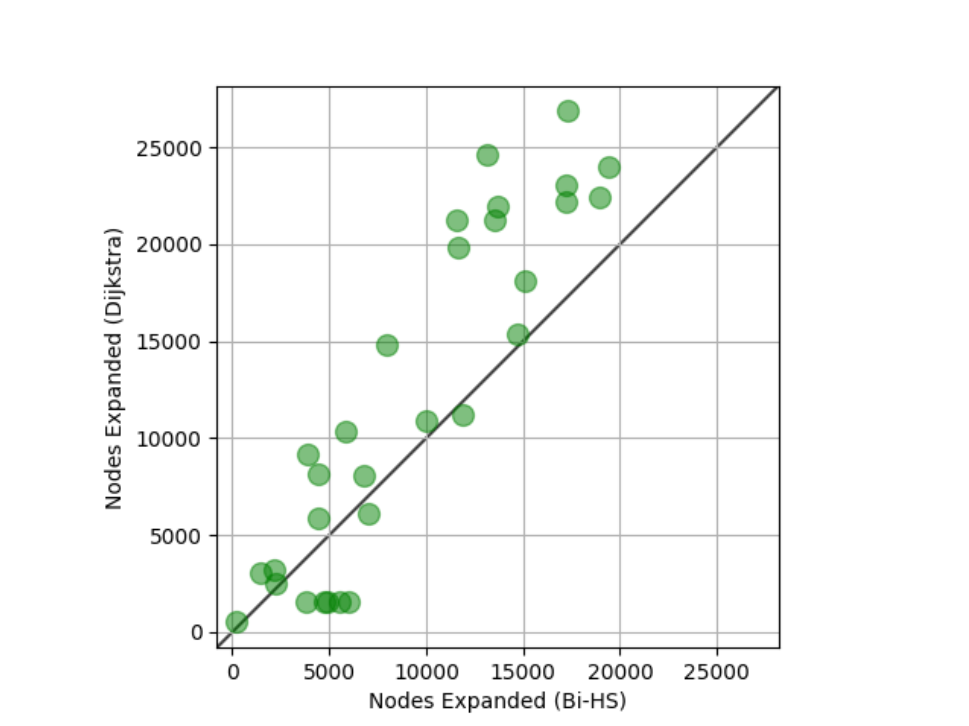
\includegraphics[width=\linewidth*3/6]{image.png}
    \caption{Scatter plot showing number of nodes expanded for Dijkstra vs number of nodes expanded for Bi-BS for all test cases}
  \end{center}
\end{figure}
\begin{enumerate}
  \item Why is the overall distribution of points in the plot the way it is?\\
<<<<<<< HEAD
    The overall distribution of points in the plot are above the line meaning that in most cases, more nodes are expanded in the Dijkstra implementation compared to the Bi-BS implementation. The number of states in Dijkstra's algorithm can exponentially grow with the search depth until it finds the solution depth $C*$. In Bi-BS, we simultaneously search from the goal and start and the solution is found when the searches "meet in the middle". The solution depth for the start or goal in Bi-BS does not expand nodes with cost larger than $C*/2$, so it is not as large as that of Dijkstra for the same problem.
=======
    The overall distribution of points in the plot are above the line meaning that in most cases, more nodes are expanded in the Dijkstra implementation compared to the Bi-BS implementation. The number of states in Dijkstra's algorithm can exponentially grow with the search depth until it finds the solution depth $C*$. In Bi-BS, we simultaneously search from the goal and start and the solution is found when the searches meet in the middle. The solution depth for the start or goal in Bi-BS does not expand nodes with cost larger than $C*/2$, so it is not as large as that of Dijkstra for the same problem.
>>>>>>> 05d5fc7504790d11cd84bd8aa2d7989430b656a6
  \item Why some of the points are clearly below the main diagonal?\\
    When we plot only the points where no solution was returned, we get the following plot where all of these data points are clearly below the diagonal. 
  \begin{figure}[H]
    \begin{center}    
      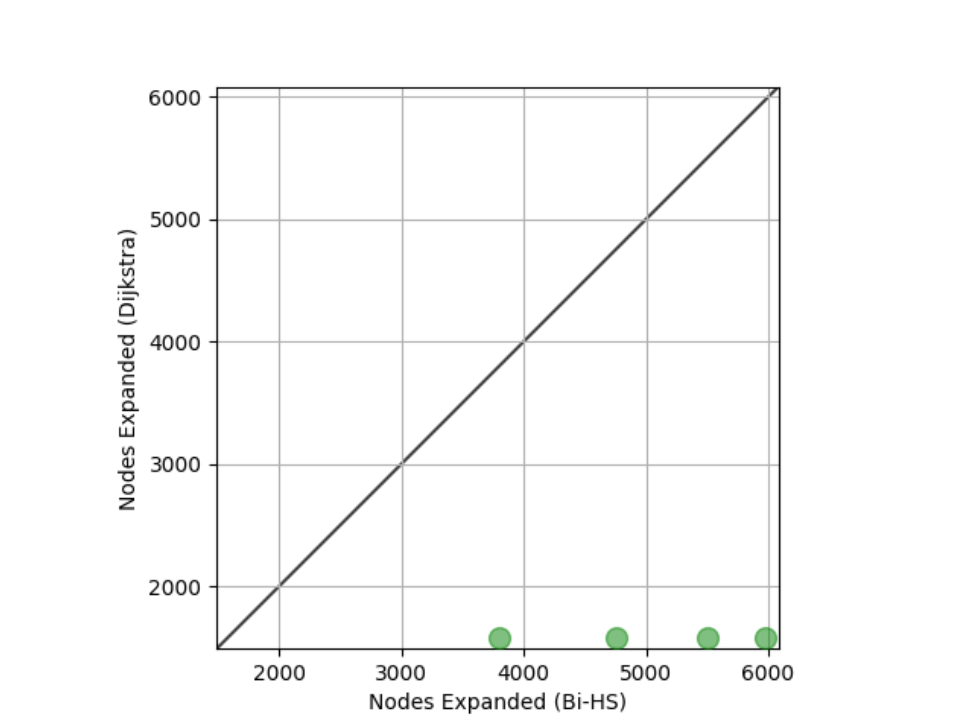
\includegraphics[width=\linewidth*3/6]{image2.png}
    \end{center}
  \end{figure}
  From the plot, we can see that for inputs with no solutions, we have more nodes expanded using Bi-BS than using Dijkstra. When we look at the specific data for some of these points more in depth, we get the following results:

  \begin{multicols}{2}  
    Dijkstra  
    \begin{lstlisting}
Start state:  [80, 229]
Goal state:  [143, 219]
Solution cost:  -1
Nodes expanded:  1577

Start state:  [112, 202]
Goal state:  [254, 153]
Solution cost:  -1
Nodes expanded:  1577
    \end{lstlisting}
    % \vfill\null
    \columnbreak
    Bi-BS
    \begin{lstlisting}
Start state:  [80, 229]
Goal state:  [143, 219]
Solution cost: -1
Nodes expanded:  4762

Start state:  [112, 202]
Goal state:  [254, 153]
Solution cost: -1
Nodes expanded:  3797
    \end{lstlisting}
  \end{multicols}
  \vspace{-0.5cm}
In Dijkstra, each input expanded exactly 1577 nodes for when all possible nodes have been expanded; however for Bi-BS, there were 2-3x more nodes expanded than in Dijkstra. This is because when there's no solution, the start and the goal expand exponentially until one side expands all possible nodes. This results in significantly more nodes to have been visited than compared to Dijkstra where there is only one search expanding all possible nodes. This means that Bi-BS is less efficient than Dijkstra when no solution exists.
\item Why some of the points are clearly above the main diagonal? \\
Most of the points are above the main diagonal because the number of nodes expanded in Dijkstra exponentially grows with search depth until it reaches the goal whereas Bi-BS grows simultaneously from the start and goal exponentially until they meet in the middle. This results in the amount of nodes seen in Bi-BS to be less than that of Dijkstra. For the points that are much higher than the diagonal line, it is possible that the start and goal were sufficiently far away from each other that Dijkstra had to search to a large depth to find the goal.
\end{enumerate}
\end{document}